\begin{enumerate}
    \item[1.1] Prove that \( \left| x \right| \leq \sum_{i=1}^n \left| x_i \right| \)
    
    \begin{proof}
    If \( \{ e_1, e_2, \ldots, e_n \} \) is the usual basis on \( \mathbb{R}^n \), then we can write
    \[
    x = x_1e_1+x_2e_2+\ldots+x_ne_n
    \]
    and thus
    \[
    \vert x \vert = \left| \sum_{i=1}^n x_ie_i \right| \leq \sum_{i=1}^n \vert x_i e_i \vert = \sum_{i=1}^n \vert x_i \vert \vert e_i \vert = \sum_{i=1}^n \vert x_i \vert
    \]
    \end{proof}
    
    \item[1.2] When does equality hold in Theorem 1-1(3)?
    
    \begin{proof}
    Notice in the proof that we get
    \[
    \vert x+y \vert^2 = \sum_{i=1}^n (x_i)^2 + \sum_{i=1}^n (y_i)^2 + 2 \sum_{i=1}^n x_iy_i \leq \vert x \vert^2 + \vert y \vert^2 +2\vert x \vert \vert y \vert
    \]
    and so we have equality precisely when \( \sum_{i=1}^n x_iy_i = \left| \sum_{i=1}^n x_iy_i \right|\) and \( x \) and \( y \) are dependent. That is, when \( x \) and \( y\) are dependent and \( sgn(x_i) = sgn(y_i) \) for all \( i \). That is, when one is a non-negative multiple of the other.
    \end{proof}
    
    \item[1.3] Prove that \( \vert x-y \vert \leq \vert x \vert + \vert y \vert \). When does equality hold?
    
    \begin{proof}
    \[
    \vert x-y \vert = \vert x + (-y) \vert \leq \vert x \vert + \vert -y \vert = \vert x \vert + \vert y \vert
    \]
    Conditions for equality are the same as in 1.2, for \( x \) and \( -y \). 
    \end{proof}
    
    \item[1.4] Prove that \( \left| \vert x \vert - \vert y \vert \right| \leq \vert x-y \vert \).
    
    \begin{proof}
    Notice
    \[
    \vert x \vert = \vert x - y +y \vert \leq \vert x-y \vert + \vert y \vert 
    \]
    Thus
    \[
    \vert x \vert - \vert y \vert \leq \vert x-y \vert
    \]
    Similarly,
    \[
    \vert y \vert = \vert y-x+x \vert \leq \vert y-x \vert + \vert x \vert = \vert x-y \vert + \vert x \vert
    \]
    Thus
    \begin{align*}
        \vert y \vert - \vert x \vert &\leq \vert x-y \vert \\
        -\vert x-y \vert &\leq \vert x \vert - \vert y \vert
    \end{align*}
    So, combining these results yields
    \[
    -\vert x-y \vert \leq \vert x \vert - \vert y \vert \leq \vert x-y \vert
    \]
    which implies
    \[
    \left| \vert x \vert - \vert y \vert \right| \leq \vert x-y \vert
    \]
    as desired.
    \end{proof}
    
    \item[1.5] The quantity \( \vert y -x \vert \) is called the \textbf{distance} between \( x \) and \( y \). Prove and interpret geometrically the ``triangle inequality":
    \[
    \vert z-x \vert \leq \vert z-y \vert + \vert y-x \vert
    \]
    
    \begin{proof}
    \[
    \vert z-x \vert = \vert z-y+y-x \vert \leq \vert z-y \vert + \vert y-x \vert
    \]
    Geometrically, we have
    \begin{center}
    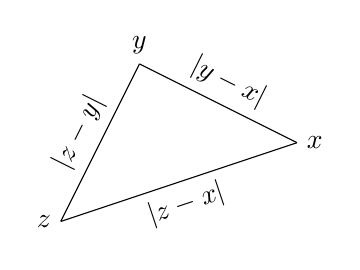
\begin{tikzpicture}
    \coordinate [label=left:$z$] (z) at (0,0);
    \coordinate [label=above:$y$] (y) at (1,2);
    \coordinate [label=right:$x$] (x) at (3,1);
    
    \draw (z) -- (y) node [midway, above, sloped] (TextNode) {$\vert z-y \vert$};
    \draw (y) -- (x) node [midway, above, sloped] (TextNode) {$\vert y-x \vert$};
    \draw (x) -- (z) node [midway, below, sloped] (TextNode) {$\vert z-x \vert$};
    \end{tikzpicture}
    \end{center}
    \end{proof}
    
    \item[1.6] Let \( f \) and \( g \) be integrable on \( [a,b] \).
    \begin{enumerate}
        \item Prove that \( \left| \int_a^b f\cdot g \right| \leq \left( \int_a^b f^2 \right)^{\frac{1}{2}} \cdot \left( \int_a^b g^2 \right)^{\frac{1}{2}}  \).
        \item If equality holds, must \( f = \lambda g \) for some \( \lambda \in \mathbb{R} \)? What if \( f \) and \( g \) are continuous?
        \item Show that Theorem 1-1(2) is a special case of (a).
    \end{enumerate}
    
    \begin{proof}
    \begin{enumerate}
        \item One way to prove this would be to observe that 1-1(2) implies that
        \[
        \left| \sum_{k=1}^n f(t_k)g(t_k)\Delta x_k \right| \leq \left( \sum_{k=1}^n (f(t_k))^2\Delta x_k \right)^{\frac{1}{2}} \left( \sum_{k=1}^n (g(t_k))^2 \Delta x_k \right)^{\frac{1}{2}}
        \]
        Notice, by integrability, all the sums can be considered functions of the tagged partition \( \dot{\mathcal{P}} \), such that each will approach \( \int_a^b f\cdot g \), \( \int_a^b f^2 \) and \( \int_a^b g^2 \), respectively, when \( \left|\left| \dot{\mathcal{P}} \right|\right| \rightarrow 0 \). Thus, by continuity of the square root function and the absolute value, taking the limit as \( \left|\left| \dot{\mathcal{P}} \right|\right| \rightarrow 0 \) will give us the desired result. 
        
        \hfill
        
        However, following Spivak's hint, we observe that either there exists \( \lambda \in \mathbb{R} \) such that
        \[
        0 = \int_a^b (f-\lambda g)^2
        \]
        or, since \( (f-\lambda g)^2 \) is nonnegative, for all \( \lambda \in \mathbb{R} \)
        \[
        0 < \int_a^b (f-\lambda g)^2
        \]
        Notice from Lebesgue's theorem of Riemann-integrability that in the first case we must have that \( f=\lambda g \) almost everywhere on \( [a,b] \), and therefore
        \begin{align*}
            \int_a^b f\cdot g &= \lambda \int_a^b g^2 \\
            \intertext{and}
            \int_a^b f^2 &= \int_a^b \lambda^2 g^2
        \end{align*}
        Which would give us that
        \[
        \left| \int_a^b f\cdot g \right| = \left| \lambda \int_a^b g^2 \right| = \sqrt{\lambda^2 \left(\int_a^b g^2\right)^2} = \sqrt{\int_a^b \lambda^2 g^2 \int_a^b g^2} = \sqrt{\int_a^b f^2 \int_a^b g^2 }
        \]
        which can be rewritten as
        \[
        \left| \int_a^b f\cdot g \right| = \left( \int_a^b f^2 \right)^{\frac{1}{2}} \left( \int_a^b g^2 \right)^{\frac{1}{2}}
        \]
        In the second case, we have that
        \[
        0 < \int_a^b (f-\lambda g)^2 = \int_a^b f^2 -2\lambda \int_a^b f\cdot g + \lambda^2 \int_a^b g^2
        \]
        On the right, we have a quadratic in \( \lambda \) which has no real roots since the inequality holds for all \( \lambda \in \mathbb{R} \). Thus
        \[
        4\left( \int_a^b f\cdot g \right)^2-4\int_a^b f^2 \int_a^b g^2 < 0
        \]
        which implies
        \[
        \left( \int_a^b f \cdot g \right)^2 < \int_a^b f^2 \int_a^b g^2
        \]
        which finally gives us
        \[
        -\left(\int_a^b f^2 \right)^{\frac{1}{2}} \left(\int_a^b g^2\right)^{\frac{1}{2}} < \int_a^b f \cdot g < \left(\int_a^b f^2\right)^{\frac{1}{2}} \left( \int_a^b g^2\right)^{\frac{1}{2}}
        \]
        Thus, together, the results from both cases imply that
        \[
        \left| \int_a^b f\cdot g \right| \leq \left( \int_a^b f^2 \right)^{\frac{1}{2}} \cdot \left( \int_a^b g^2 \right)^{\frac{1}{2}}
        \]
        as desired.
        
        \item No, in general, we may have \( f \neq \lambda g \) and still have \( \left| \int_a^b f\cdot g \right| = \left( \int_a^b f^2 \right)^{\frac{1}{2}} \left( \int_a^b g^2 \right)^{\frac{1}{2}} \). For example, take
        \[
        f = \begin{cases} 1, & x=1 \\ 0, & elsewhere \end{cases}
        \]
        and
        \[
        g = \begin{cases} 1, & x=0 \\ 0, & elsewhere \end{cases}
        \]
        Then \( \left| \int_0^1 f\cdot g \right| = \left( \int_0^1 f^2 \right)^{\frac{1}{2}} \left( \int_0^1 g^2 \right)^{\frac{1}{2}} = 0\) while \( f \neq \lambda g \). However, if \( f \) and \( g \) are continuous, then equality holds if and only if \( f = \lambda g \) for some \( \lambda \in \mathbb{R} \). This follows from the theorem which states that if \( f \) is continuous on \( [a,b] \) and \( f \geq 0 \) with \( f(x_0) > 0 \) for some \( x_0 \in [a,b] \) then \( \int_a^b f > 0 \). The proof of this can be found in Exercise 7.4.4 from the solutions manual for Abbott's \emph{Understanding Analysis}.
        
        \item Divide \( [a,b] \) into \( n \) sub-intervals so that on the \( i^{th} \) sub-interval, \linebreak \( \left[a+\frac{b-a}{n}(i-1), a+\frac{b-a}{n}i\right) \), we define \( f \) to be
        \[
        f(x) = \frac{x_i}{\sqrt{\frac{b-a}{n}}}
        \]
        and \( g \) to be
        \[
        g(x) = \frac{y_i}{\sqrt{\frac{b-a}{n}}}
        \]
        Then
        \begin{align*}
            \int_a^b f\cdot g &= \sum_{i=1}^n x_iy_i \\
            \int_a^b f^2 &= \sum_{i=1}^n x_i^2 \\
            \int_a^b g^2 &= \sum_{i=1}^n y_i^2
        \end{align*}
        which, by (a), gives us the desired inequality.
        
        \pagebreak
        
        \begin{table*}
        \centering
        \includegraphics[scale=0.3]{1-6Graph.jpg}
        \caption{A poorly drawn graph of \( f \)}
        \end{table*}
    \end{enumerate}
    \end{proof}
    
    \pagebreak
    
    \item[1.7] A linear transformation \( T: \mathbb{R}^n \rightarrow \mathbb{R}^n \) is \textbf{norm preserving} if \( \vert T(x) \vert = \vert x \vert \), and \textbf{inner product preserving} if \( \left< Tx, Ty \right> = \left< x,y \right> \).
    \begin{enumerate}
        \item Prove that \( T \) is norm preserving if and only if \( T \) is inner product preserving.
        
        \item Prove that such a linear transformation \( T \) is injective and \( T^{-1} \) is of the same sort.
    \end{enumerate}
    
    \begin{proof}
    \begin{enumerate}
        \item Suppose that \( T \) is norm preserving. Then, by the polarization identity, we have
        \begin{align*}
            \langle x,y \rangle &= \frac{\vert x+y \vert^2-\vert x-y \vert^2}{4} \\
            \intertext{and since \( T \) is norm preserving, we have}
            &= \frac{\vert T(x+y) \vert ^2 - \vert T(x-y) \vert ^2}{4} \\
            &= \frac{\langle T(x+y), T(x+y) \rangle - \langle T(x-y), T(x-y) \rangle}{4} \\
            \intertext{and by linearity of \( T \), we have}
            &= \frac{\langle T(x) + T(y), T(x) + T(y) \rangle - \langle T(x) - T(y), T(x) - T(y) \rangle}{4} \\
            \intertext{and by bilinearity of the inner product, we have} 
            &= \langle Tx, Ty \rangle
        \end{align*}
        
        Now, suppose that \( T \) is inner product preserving. Then
        \[
        \left| T(x) \right| = \sqrt{\langle T(x), T(x) \rangle} = \sqrt{\langle x, x \rangle} = \vert x \vert
        \]
        
        \item Suppose that \( T \) is norm preserving (and therefore, also inner product preserving) and that
        \begin{align*}
            T(x) &= T(y)\\
            \intertext{then}
            T(x) - T(y) &= 0 \\
            T(x-y) &= 0 \\
            \left| T(x-y) \right| &= 0 \\
            \left| x-y \right| &= 0 \\
            \intertext{which implies that}
            x-y &= 0 \\
            x &= y
        \end{align*}
        Therefore, \( T \) is injective. Since injectivity of a linear transformation is equivalent to surjectivity, it follows that \( T^{-1} \) exists. To show that \( T^{-1} \) is of the same sort, we show that it is norm preserving. Observe that
        \[
        \left| T^{-1}(y) \right| = \left| x \right| = \left| T(x) \right| = \left| y \right|
        \]
    \end{enumerate}
    \end{proof}
    
    \item[1.8] If \( x,y \in \mathbb{R}^n \) are non-zero, the \textbf{angle} between \( x \) and \( y \), denoted \( \angle(x,y) \), is defined as \( \arccos \left( \frac{\langle x, y \rangle}{\vert x \vert \cdot \vert y \vert} \right) \), which makes sense by Theorem 1-1(2). The linear transformation \( T \) is \textbf{angle preserving} if \( T \) is injective, and for \( x,y \neq 0 \) we have \( \angle(Tx,Ty) = \angle(x,y) \).
    \begin{enumerate}
        \item Prove that if \( T \) is norm preserving, then \( T \) is angle preserving.
        
        \item If there is a basis \( x_1, \ldots, x_n \) of \( \mathbb{R}^n \) and numbers \( \lambda_1, \ldots, \lambda_n \) such that \( Tx_i = \lambda_i x_i \), prove that \( T \) is angle preserving if and only if all \( \vert \lambda_i \vert \) are equal.
        
        \item What are all angle preserving \( T: \mathbb{R}^n \rightarrow \mathbb{R}^n \)?
    \end{enumerate}
    
    \begin{proof}
    \begin{enumerate}
        \item If \( T \) is norm preserving, then it is also inner product preserving and injective. Thus, if \( x, y \neq 0 \),
        \[
        \angle(Tx, Ty) = \arccos\left( \frac{\langle Tx, Ty \rangle}{\vert Tx \vert \cdot \vert Ty \vert} \right) = \arccos\left( \frac{\langle x, y \rangle}{\vert x \vert \cdot \vert y \vert} \right) = \angle(x,y)
        \]
        so that \( T \) is also angle preserving.
        
        \item This is not true. Take \( ( (-1,-1), (1,0) ) = (x_1, x_2) \) as a basis for \( \mathbb{R}^2 \). If 
        \begin{align*}
            T(x_1) &= 3x_1 \\
            T(x_2) &= -3x_2
        \end{align*}
        Then \( T \) is injective and has that \( \vert \lambda_i \vert \) are all equal. However,
        \begin{align*}
            \angle(x_1,x_2) &= \frac{3\pi}{4} \\
            \intertext{while}
            \angle(Tx_1, Tx_2) &= \frac{\pi}{4}
        \end{align*}
    \end{enumerate}
    \end{proof}
    
    \item[1.9] If \( 0 \leq \theta < \pi \), let \( T: \mathbb{R}^2 \rightarrow \mathbb{R}^2 \) have the matrix 
    \[
    \begin{bmatrix}
    \cos \theta & \sin \theta \\
    -\sin \theta & \cos \theta
    \end{bmatrix}
    \]
    Show that \( T \) is angle preserving and if \( x \neq 0 \), then \( \angle (x,Tx) = \theta \). 
    
    \begin{proof}
    Observe that
    \begin{align*}
        \begin{bmatrix} \cos \theta & \sin \theta \\ -\sin \theta & \cos \theta \end{bmatrix} \begin{bmatrix} x_1 \\ x_2 \end{bmatrix} &= \begin{bmatrix} x_1 \cos \theta + x_2 \sin \theta \\ -x_1 \sin \theta + x_2 \cos \theta \end{bmatrix} \\
        \intertext{and}
        \begin{bmatrix} \cos \theta & \sin \theta \\ -\sin \theta & \cos \theta \end{bmatrix} \begin{bmatrix} y_1 \\ y_2 \end{bmatrix} &= \begin{bmatrix} y_1 \cos \theta + y_2 \sin \theta \\ -y_1 \sin \theta + y_2 \cos \theta \end{bmatrix}
    \end{align*}
    Now, some rather tedious calculations show that
    \[
        \langle Tx, Ty \rangle = x_1y_1 + x_2y_2 = \langle x, y \rangle
    \]
    and
    \[
        \left| Tx \right| = \left| x \right|
    \]
    and
    \[
        \left| Ty \right| = \left| y \right|
    \]
    which, together, imply that \( \angle (Tx, Ty) = \angle (x,y) \) so that \( T \) is angle preserving. Again, a rather tedious calculation shows that
    \[
    \langle x, Tx \rangle = \left| x \right|^2 \cos \theta
    \]
    which implies that, for \( x \neq 0 \)
    \begin{align*}
        \angle(x, Tx) &= \arccos \left( \frac{\langle x, Tx \rangle}{\left| x \right| \cdot \left| Tx \right|} \right) \\
        &= \arccos \left( \frac{\left| x \right|^2 \cos \theta}{\left| x \right|^2} \right) \\
        &= \arccos (\cos \theta) \\
        &= \theta
    \end{align*}
    \end{proof}
    
    \item[1.10\(^*\)] If \( T: \mathbb{R}^m \rightarrow \mathbb{R}^n \) is a linear transformation, show that there is a number \( M \) such that \( \left| T(h) \right| \leq M \left| h \right| \) for \( h \in \mathbb{R}^m \). 
    
    \begin{lemma}
    Let \( T \in \mathcal{L}(\mathbb{R}^m, \mathbb{R}^n) \). Then there exists \( M>0 \) such that for all \( x \) admitting \( \left| x \right| = 1 \), we have
    \[
    \left| T(x) \right| \leq M
    \]
    \end{lemma}
    
    \begin{proof}[Proof of Lemma]
    Let \( \left| x \right| = 1 \). Given the standard basis, \( \{e_1, \ldots, e_m \} \), on \( \mathbb{R}^m \) we may write
    \[
    x = \alpha_1 e_1 + \ldots + \alpha_m e_m
    \]
    where \( \left| \alpha_i \right| \leq 1 \) for all \( 1 \leq i \leq m \). Thus
    \begin{align*}
        \left| T(x) \right| &= \left| T(\alpha_1 e_1 + \ldots + \alpha_m e_m) \right| \\
        &= \left| \alpha_1T(e_1) + \ldots + \alpha_m T(e_m) \right| \\
        &\leq \left| \alpha_1 \right| \left| T(e_1) \right| + \ldots + \left| \alpha_m \right| \left| T(e_m) \right| \\
        &\leq \left| T(e_1) \right|+\ldots+\left| T(e_m) \right| \\
        &= M
    \end{align*}
    \end{proof}
    
    \begin{proof}[Proof of 1.10]
    From the Lemma, we get that there exists \( M > 0 \) such that, if \( h \neq 0 \), then
    \begin{align*}
        \left| T\left( \frac{h}{\left| h \right|} \right) \right| & \leq M \\
        \left| \frac{1}{\left| h \right|} T(h) \right| &\leq M \\
        \left| T(h) \right| &\leq M \left| h \right|
    \end{align*}
    \end{proof}
    
    \item[1.11] If \( x,y \in \mathbb{R}^n \) and \( z,w \in \mathbb{R}^m \), show that \( \langle (x,z), (y,w) \rangle = \langle x,y \rangle + \langle z,w \rangle \) and \( \left| (x,z) \right| = \sqrt{\left| x \right|^2 + \left| z \right|^2} \). Note that \( (x,z) \) and \( (y,w) \) denote points in \( \mathbb{R}^{n+m} \). 
    
    \begin{proof}
    Observe
    \[
    (x,z) = (x_1,\ldots, x_n,z_1,\ldots,z_m)
    \]
    and
    \[
    (y,w) = (y_1,\ldots,y_n,w_1,\ldots,w_m)
    \]
    and thus
    \[
    \langle (x,z), (y,w) \rangle = \sum_{i=1}^n x_iy_i + \sum_{i=1}^m z_iw_i = \langle x, y \rangle + \langle z,w \rangle
    \]
    and
    \[
    \left| (x,z) \right| = \sqrt{\sum_{i=1}^n x_i^2 + \sum_{i=1}^m z_i^2} = \sqrt{\left| x \right|^2 + \left| z \right|^2}
    \]
    \end{proof}
    
    \item[1.12\(^*\)] Let \( \left( \mathbb{R}^n \right)^* \) denote the dual space of the vector space \( \mathbb{R}^n \). If \( x \in \mathbb{R}^n \), define \( \phi_x \in \left( \mathbb{R}^n \right)^* \) by \( \phi_x(y) = \langle x, y \rangle \). Define \( T: \mathbb{R}^n \rightarrow \left( \mathbb{R}^n \right)^* \) by \( T(x) = \phi_x \). Show that \( T \) is an injective linear transformation and conclude that every \( \phi \in \left( \mathbb{R}^n \right)^* \) is \( \phi_x \) for a unique \( x \in \mathbb{R}^n \).
    
    \begin{proof}
    The linearity of the inner product implies the linearity of \( T \). To show that \( T \) is injective, by linearity of \( T \), it is sufficient to show that \( ker(T) = \{0 \} \). To that end, suppose that
    \begin{align*}
        T(x) &= 0 \\
        \intertext{then}
        \phi_x &= 0
        \intertext{so that}
        \phi_x(x) &= 0 \\
        \langle x, x \rangle &= 0
        \intertext{if and only if}
        x &= 0
    \end{align*}
    Thus \( ker(T) = \{ 0 \} \) and \( T \) is injective. Moreover, since \( \dim(\mathbb{R}^n)^* = \dim\mathbb{R}^N \), injectivity of \( T \) implies surjectivity. Thus \( T \) is a bijection between \( \mathbb{R}^n \) and \( (\mathbb{R}^n)^* \). Thus each \( \phi \in \left( \mathbb{R}^n \right)^* \) corresponds to a \( \phi_x \) for some unique \( x \in \mathbb{R}^n \).   
    \end{proof}
    
    \item[1.13\(^*\)] If \( x,y \in \mathbb{R}^n \), then \( x \) and \( y \) are called \textbf{perpendicular} (or \textbf{orthogonal}) if \( \langle x, y \rangle = 0 \). If \( x \) and \( y \) are perpendicular, prove that 
    \[
    \left| x + y \right|^2 = \left| x \right|^2 + \left| y \right|^2
    \]
    \begin{proof}
    \[
    \left| x+y \right|^2 = \langle x+y, x+y \rangle = \langle x,x \rangle + 2\langle x, y \rangle + \langle y, y \rangle = \langle x,x \rangle + \langle y, y \rangle = \left| x \right|^2 + \left| y \right|^2
    \]
    \end{proof}
    
    \item[1.14\( ^*\)] Prove that the union of any (even infinite) number of open sets is open. Prove that the intersection of two (and hence infinitely many) open sets is open. Give a counterexample for infinitely many open sets.
    
    \begin{proof}
    Let \( x \in \cup_\lambda O_\lambda \) with each \( O_\lambda \) open. Then there exists \( \lambda \) such that \( x \in O_\lambda \). Since \( O_\lambda \) is open, there exists an open rectangle, \( A \), such that \( x \in A \subset O_\lambda \subset \cup_\lambda O_\lambda \). Thus the arbitrary union of open sets is open. A simple but tedious argument could be made to show that the intersection of two open rectangles is, again, an open rectangle. Then the intersection of two open sets being, again open is a simple corollary. Notice that
    \[
    \bigcap_{n=1}^\infty \left( -\frac{1}{n}, \frac{1}{n} \right) = \{ 0 \}
    \]
    Clearly, \( \{ 0 \} \) does not contain any open rectangles, and is therefore not open. 
    \end{proof}
    
    \item[1.15] Prove that \( \{ x \in \mathbb{R}^n : \left| x-a \right| < r \}\) is open.
    
    \begin{lemma}
    There exists an open rectangle, \( U \), such that \( U \subset B_0(r)=\{ x \in \mathbb{R}^n: \left| x \right| < r \} \)
    \end{lemma}
    
    \begin{proof}
    Let \( U = \Pi_{i=1}^n (-\frac{\epsilon}{\sqrt{n}}, \frac{r}{\sqrt{n}})  \). Then
    \[
    \left| x \right|^2 \leq \sum_{i=1}^n \left|x_i\right|^2 < \sum_{i=1}^n \left(\frac{r}{\sqrt{n}}\right)^2 = r^2
    \]
    implying \( \left| x \right| < r \). Therefore \( U \subset B_0(r) \). 
    \end{proof}
    
    \textbf{Corollary.} There exists an open rectangle, \( U \), such that \( U \subset B_a(r) = \{ x\in \mathbb{R}^n: \left| x-a \right| < r \} \) is open.
    
    \begin{proof}
    By the transformation \( T(x) = x-a \) and the open rectangle \( U \) from the Lemma. 
    \end{proof}
    
    \textbf{Corollary.} \( B_a(r) \) is open.
    
    \begin{proof}
    Let \( x \in B_a(r) \). Then, from the Corollary, we get that there exists an open rectangle, \( U \), such that
    \[
    U \subset B_x\left( r-\left| x-a \right|\right) \subset B_a(r)
    \]
    Therefore, \( B_a(r) \) is open.
    \end{proof}
    
    It is not to hard to apply the same idea backwards: every open rectangle contains an open ball. Thus a set, \( A \), is open if and only if for each \( x \in A \) there exists \( B_x(r) \) such that \( B_x(r) \subset A \). This characterization of open sets is often easier to work with than the characterization provided in the book. We will consider this as given for future exercises.
    
    \item[1.16] Find the interior, exterior, and boundary of the sets.
    \begin{center}
    \( \{ x \in \mathbb{R}^n : \left| x \right| \leq 1 \} \)
    
    \( \{ x \in \mathbb{R}^n : \left| x \right| = 1 \} \)
    
    \( \{ x \in \mathbb{R}^n : \text{ each } x_i \text{ is rational.} \} \)
    \end{center}
    
    \begin{proof}
    For the first, we have that the interior is \( \{ x \in \mathbb{R}^n: \left| x \right| < 1 \} \), the exterior is \( \{ x \in \mathbb{R}^n : \left| x \right| > 1 \} \), and the boundary is \( \{ x \in \mathbb{R}: \left| x \right| = 1 \} \).
    
    For the second, we have that the interior is empty (every open rectangle in \( \mathbb{R}^n \) will contain some points outside this set), the exterior is \( \{ x \in \mathbb{R}^n: \left| x \right| \neq 1 \} \), and the boundary is the set itself.
    
    For the third, we have that both the interior and exterior are empty, and the boundary is again the set itself.
    \end{proof}
    
    \item[1.17] Construct a set \( A \subset [0,1] \times [0,1] \) such that \( A \) contains at most one point on each horizontal and each vertical line but boundary \( A = [0,1] \times [0,1] \). 
    
    \begin{proof}
    Let \( A \) be the set of all points with rational coordinates in \( (0,1) \times (0,1) \). Then clearly \( boundary(A) \subset [0,1] \times [0,1] \). If \( x \in [0,1] \times [0,1] \) then \( x = (x_1, x_2) \) where \( 0 \leq x_1, x_2 \leq 1 \). Thus, if \( B \) is an open set containing \( x \), it follows that there exist \( 0 \leq \epsilon_1, \epsilon_2 \) such that \( [x_1-\epsilon_1, x_1+\epsilon_1] \times [x_2-\epsilon_2, x_2+\epsilon_2] \subset B \cap [0,1] \times [0,1] \). Density of \( \mathbb{Q} \) in \( \mathbb{R} \) and the existence of an irrational between any two reals implies that \( [0,1] \times [0,1] \subset boundary(A) \). Thus \( boundary(A) = [0,1] \times [0,1] \).
    \end{proof}
    
    \item[1.18] If \( A \subset [0,1] \) is the union of open intervals \( (a_i,b_i) \) such that each rational number in \( (0,1) \) is contained in some \( (a_i,b_i) \), show that \( boundary(A) = [0,1] \setminus A \).
    
    \begin{proof}
    Notice, by openness of \( A \), \( x \in boundary(A) \) implies \( x \not\in A \). Furthermore, by openness of \( [0,1]^c \), \( x \in boundary (A) \) implies \( x \not\in [0,1]^c \). If \( x \in [0,1] \setminus A \) and if \( B \) is open with \( x \in B \), then \( B \cap A^c \neq \emptyset \). Furthermore, by density of \( \mathbb{Q} \) in \( \mathbb{R} \) we also get that there exists a rational \( r \in B \cap A \), so that \( B \cap A \neq \emptyset \). Thus \( boundary(A) = [0,1] \setminus A \). 
    \end{proof}
    
    \item[1.19\(^*\)] If \( A \) is a closed set that contains every rational number \( r \in [0,1] \), show that \( [0,1] \subset A \)
    
    \begin{proof}
    Suppose, to the contrary, that there exists \( x \in [0,1] \cap A^c \). Since \( A \) is closed, it follows that \( A^c \) is open and that therefore, there exists an open \( B \) such that \( x \in B \subset A^c \). But, by density of \( \mathbb{Q} \) in \( \mathbb{R} \), we know that there exists a rational \( r \in A \cap B \) contradicting with \( B \subset A^c \). Thus \( [0,1] \subset A \). 
    \end{proof}
    
    \item[1.20] Show that a compact set in \( \mathbb{R}^n \) is closed and bounded.
    
    \begin{proof}
    If \( K \subset \mathbb{R}^n \) is compact then clearly it is bounded, for if it were unbounded, then \( \{ \Pi_1^n (-k,k) : k \in \mathbb{N} \} \) would be an open cover of \( K \) which admits no finite subcover. To show that \( K \) is closed, let \( x \in K^c \) and consider the open cover of \( K \) given by
    \[
    \left\{ B_k\left( \frac{\left| x-k \right|}{2} \right): k \in K \right\}
    \]
    By compactness, there exists a finite subcover
    \[
    \left\{ B_{k_i}\left( \frac{\left| x-k_i \right|}{2} \right): 1 \leq i \leq n \right\}
    \]
    Thus \( B_x\left( \frac{\min_i \left| x-k_i \right|}{2} \right) \subset K^c \). Therefore, \( K^c \) is open. 
    \end{proof}
    
    \item[1.21\(^*\)] \begin{enumerate}
        \item If \( A \) is closed and \( x \not\in A \), prove that there is a number \( d > 0 \) such that \( \left| y -x \right| \geq d \) for all \( y \in A \).
        
        \item If \( A \) is closed, \( B \) is compact, and \( A \cap B = \emptyset \), prove that there is \( d > 0 \) such that \( \left| y - x \right| \geq d \) for all \( y \in A \) and \( x \in B \).
        
        \item Give a counterexample in \( \mathbb{R}^2 \) if \( A \) and \( B \) are closed but neither is compact.
    \end{enumerate}
    
    \begin{proof}
    \begin{enumerate}
        \item Let \( A \) be closed and \( x \in A^c \). Since \( A \) is closed, there exists an open \( B \subset A^c \) with \( x \in B \). So there exists an open ball \( B_x(r) \subset A^c \). Thus, if \( y \in A \), then \( y \in \left( B_x(r) \right)^c \). Thus
        \[
        \left| y - x \right| \geq r 
        \]
        
        \item Let \( A \) be closed and \( B \) be compact with \( A \cap B = \emptyset \). Since \( A \) is closed and \( A \) and \( B \) are disjoint, by (a), we know that for every \( x \in B \) there exists \( d_x > 0 \) such that for all \( y \in A \) we have \( \left| y-x \right| \geq d_x \). So
        \[
        \left\{ B_x\left( \frac{d_x}{2} \right): x \in B \right\}
        \]
        forms an open cover of \( B \). By compactness of \( B \), there exists a finite subcover
        \[
        \left\{ B_{x_1}\left( \frac{d_{x_1}}{2} \right), \ldots,B_{x_m}\left( \frac{d_{x_m}}{2} \right) \right\}
        \]
        So for all \( y \in A \) and \( 1 \leq i \leq m \)
        \[
        \left| y - x_i \right| \leq \left| y - x \right| + \left| x - x_i \right|
        \]
        Thus, if \( x \in B \) then \( x \in B_{x_i}\left( \frac{d_{x_i}}{2} \right) \) for some \( i \), and the above inequality implies 
        \[
        \min_{1 \leq i \leq m} \frac{d_{x_i}}{2} \leq \frac{d_{x_i}}{2} = d_{x_i} - \frac{d_{x_i}}{2} \leq \left| y-x_i \right| - \left| x - x_i  \right| \leq \left| y - x \right| 
        \]
        \item If
        \begin{align*}
            A &= \left\{ (0, n): n \in \mathbb{N} \right\} \\
            \intertext{and}
            B &= \left\{ (0, n-\frac{1}{n}): n \in \mathbb{N} \right\}
        \end{align*}
        then it is clear that both \( A \) and \( B \) are closed, but not bounded and therefore not compact. Furthermore, \( A \cap B = \emptyset \) and for all \( n \in \mathbb{N} \) we can find \( y \in A \) and an \( x \in B \) such that
        \[
        \left| y-x \right| < \frac{1}{n}
        \]
    \end{enumerate}
    \end{proof}
    
    \item[1.22\( ^* \)] If \( U \) is open and \( C \subset U \) is compact, show that there is a compact set \( D \) such that \( C \subset interior(D) \) and \( D \subset U \).
    
    \begin{proof}
    Let \( U \) be open and \( C \subset U \) be compact. It follows that \( U^c \) is closed and that \( U^c \cap C = \emptyset \). By the previous exercise, we know then that there exists a \( d > 0 \) such that
    \[
    \left| x-y \right| \geq d
    \]
    for all \( x \in C \) and \( y \in U^c \). We observe that since
    \[
    \{ B_x(d/2): x \in C \}
    \]
    forms an open cover of \( C \), there is a finite subcover \( \{ B_{x_1}, \ldots, B_{x_m} \} \). So if we denote
    \[
    \overline{B_x(d/2)} = \left\{ z: \left| x-z \right| \leq \frac{d}{2} \right\}
    \]
    then 
    \[
    \bigcup_{i=1}^m \overline{B_{x_i}(d/2)} = D
    \]
    is compact and
    \[
    C \subset D \subset U
    \]
    If \( x \in C \) then it follows \( x \in B_x(d/2) \subset D \) which implies \( C \subset Int(D) \)
    \end{proof}
    
    \item[1.23] If \( f: A \rightarrow \mathbb{R}^m \) and \( a \in A \), show that \( \lim_{x \rightarrow a} f(x) =b \) if and only if \( \lim_{x \rightarrow a} f_i(x)=b_i \) for \( 1 \leq i \leq m \).
    
    \begin{proof}
    We first show sufficiency by contrapositive. Suppose that there is \( 1 \leq k \leq m \) such that
    \[
    \lim_{x \rightarrow a} f_k(x) \neq b_k
    \]
    Then there is a sequence \( (x_r) \subset A \setminus \{ a \} \) and \( \epsilon > 0 \) such that \( x_r \rightarrow a \) and for all \( r \in \mathbb{N} \) we have
    \[
    \left| f_k(x_r)-b_k \right| \geq \epsilon
    \]
    which, in turn, implies
    \[
    (f_k(x_r)-b_k)^2 \geq \epsilon^2
    \]
    Thus, for the same \( \epsilon \) we have that for every \( \delta > 0 \) there is \( r \in \mathbb{N} \) such that \( 0 < \left| x_r - a \right| < \delta \) while
    \[
    \left| f(x_r) - b \right|^2 = \sum_{i=1}^m (f_k(x_r)-b_k)^2 \geq \sum_{\substack{i=1 \\ i\neq k}}^m (f_k(x_r)-b_k)^2 + \epsilon^2 \geq \epsilon^2
    \]
    which implies that for all \( \delta > 0 \) there exists \( r \in \mathbb{N} \) such that \( 0 < \left| x_r - a \right| < \delta \) while
    \[
    \left| f(x_r) - b \right| \geq \epsilon
    \]
    so that \( \lim_{x \rightarrow a} f(x) \neq b \). To demonstrate necessity, let 
    \[
    \lim_{x\rightarrow a} f_i(x) = b_i
    \]
    for every \( 1 \leq i \leq m \). Given \( \epsilon > 0 \), we may choose \( \delta > 0 \) so that \( 0 < \left| x-a \right| < \delta \) implies
    \[
    \left| f_i(x)-b_i \right| < \frac{\epsilon}{m}
    \]
    for every \( 1 \leq i \leq m \). Thus for \( 0 < \left| x-a \right| < \delta \) we have
    \[
    \left| f(x) - b \right| \leq \sum_{i=1}^m \left| f_i(x)-b_i \right| \leq \sum_{i=1}^m \frac{\epsilon}{m} = \epsilon
    \]
    Therefore,
    \[
    \lim_{x\rightarrow a} f(x) = b
    \]
    \end{proof}
    
    \item[1.24] Prove that \( f: A \rightarrow \mathbb{R}^m \) is continuous at \( a \) if and only if each \( f_i \) is.
    
    \begin{proof}
    Notice \( f \) is continuous at \( a \) if and only if \( \lim_{x \rightarrow a} f(x) = f(a) \) if and only if \( \lim_{x \rightarrow a} f_i(x) = f_i(a) \) for every \( 1 \leq i \leq m \). 
    \end{proof}
    
    \item[1.25] Prove that a linear transformation \( T: \mathbb{R}^n \rightarrow \mathbb{R}^m \) is continuous.
    
    \begin{proof}
    From 1.10 we know that there exists an \( M >0 \) such that
    \[
    \left| T(h) \right| \leq M \left| h \right|
    \]
    So, if \( \epsilon > 0 \) is given, and \( h \in \mathbb{R}^n \) then whenever \( 0 < \left| x-h \right| < \frac{\epsilon}{M} \) we get that
    \[
    \left| T(x) - T(h) \right| = \left| T(x-h) \right| \leq M \left| x-h \right| < M \frac{\epsilon}{M} = \epsilon
    \]
    Therefore \( T \) is continuous. 
    \end{proof}
    
    \item[1.26] Let \( A = \{ (x,y)\in \mathbb{R}^2: x>0 \text{ and } 0<y<x^2 \} \)
    \begin{enumerate}
        \item Show that every straight line through \( (0,0) \) contains an interval around \( (0,0) \) which is in \( A^c \).
        \item Define \( f:\mathbb{R}^2 \rightarrow \mathbb{R} \) by \( f(x) = 0 \) if \( x \not\in A \) and \( f(x) =1 \) if \( x \in A \). For \( h \in \mathbb{R}^2 \) define \( g_h: \mathbb{R} \rightarrow \mathbb{R} \) by \( g_h(t) = f(th) \). Show that each \( g_h \) is continuous at \( 0 \), but \( f \) is not continuous at \( (0,0) \).
    \end{enumerate}
    
    \begin{proof}
    \begin{enumerate}
        \item Let \( s \) be a straight line through \( (0,0) \). If \( s \) is just the vertical line through \( x=0 \) then \( s \subset A^c \). Similarly, if \( s(x) = mx \) with \( m \leq 0 \) then \( s \subset A^c \). If \( s(x) = mx \) with \( m>0 \) , then  \( \{ (x,mx) : x\leq m \} \subset s \cap A^c \).
        
        \item First, we demonstrate that \( f \) is not continuous at \( (0,0) \). Observe that \( f((0,0)) = 0 \). Notice that the sequence \( \left( \frac{1}{n}, \frac{1}{n} \right) \rightarrow (0,0) \) and yet \( f\left( \left( \frac{1}{n}, \frac{1}{n} \right) \right) = 1 \) for all \( n \) implying that \( f \) is not continuous at \( (0,0) \). Now, if \( h \) is of the form \( (0,h_2) \) then \( g_h(t) = 0 \) and is therefore continuous at \( 0 \). If \( h \) is not of the form \( (0,h_2) \) then \( g_h(0) = f(0) = 0 \). Notice that \( th = t(h_1,h_2) \) is simply the line \( s(x) = \frac{h_2}{h_1}x \). By (a), we know that for \( \delta \) small enough \( f(th) = 0 \) whenever \( \vert t \vert < \delta \). Therefore \( g_h \) is continuous at \( 0 \). 
    \end{enumerate}
    \end{proof}
    
    \item[1.27] Prove that \( B_a(r) \) is open by considering the function \( f: \mathbb{R}^n \rightarrow \mathbb{R} \) with \( f(x) = \left| x-a \right| \).
    
    \textbf{Lemma.} \( \left| x \right|: \mathbb{R}^n \rightarrow \mathbb{R} \) is continuous.
    \begin{proof}[Proof of Lemma]
    Let \( \epsilon > 0 \) be given and \( c \in \mathbb{R}^n \). Then \( \left| x-c \right| < \epsilon \), along with 1.4, imply that
    \[
    \left| \left| x \right| - \left| c \right| \right| \leq \left| x-c \right| < \epsilon
    \]
    \end{proof}
    
    \textbf{Corollary.} \( f(x) = \left| x-a \right| \) is continuous.
    
    \begin{proof}[Proof of 1.27]
     Notice \( B_a(r) = f^{-1}\left( \{ f(x) \in \mathbb{R}: f(x) < r \} \right) \). Clearly \( \{ f(x) \in \mathbb{R}: 0< f(x) < r \} \) is open, so by continuity of \( f \) and definition of the norm, we have that \( B_a(r) \setminus \{ a \} \) is open. Furthermore, since \( a \in B_a(r) \subset B_a(r) \) it follows \( B_a(r) \) is open.
    \end{proof}
    
    \item[1.28] If \( A \subset \mathbb{R}^n \) is not closed, show that there is a continuous function \( f:A \rightarrow \mathbb{R} \) which is unbounded.
    
    \begin{proof}
    If \( A \) is not closed then \( A^c \) is not open and so there exists a sequence \( (a_m) \subset A \) such that \( a_m \rightarrow x \in A^c \). Thus \( f:A \rightarrow \mathbb{R} \) defined by
    \[
    f(a) = \frac{1}{\left| a-x \right|}
    \]
    is continuous and unbounded.
    \end{proof}
    
    \item[1.29] If \( A \) is compact, prove that every continuous function \( f:A \rightarrow \mathbb{R} \) takes on a maximum and minimum value.
    
    \begin{proof}
    From compactness of \( A \) and continuity of \( f \), it follows \( f(A) \) is compact. Thus \( f(A) \) is closed and bounded. Thus \( inf f(A) , sup f(A) \in f(A) \) implying \( f \) takes on a maximum and minimum value.
    \end{proof}
    
    \item[1.30] Let \( f:[a,b] \rightarrow \mathbb{R} \) be an increasing function. If \( x_1,x_2,\ldots, x_n \in [a,b] \) are distinct, show that \( \sum_{i=1}^n o(f,x_i) < f(b)-f(a) \).
    
    \begin{proof}
    Let \( x_1 < x_2 < \ldots < x_n \in [a,b] \) and let\( \delta = \frac{\min \{ \left| x_i-x_j \right|: i\neq j, 1 \leq i,j \leq n \}}{4} \). If \( 1 \leq i < n \) then, by our choice of \( \delta \), we have
    \[
    x_i + \delta < x_i + 2 \delta < x_{i+1}-\delta
    \]
    Since \( f \) is increasing, it follows
    \[
    M(x_i,f,\delta) \leq f(x_i + \delta) < f(x_i + 2 \delta) < f(x_{i+1}-\delta) \leq m(x_{i+1},f,\delta)
    \]
    which establishes that
    \[
    M(x_i,f,\delta) < m(x_{i+1},f,\delta)
    \]
    Furthermore, we observe the following
    \begin{align*}
    M(x_n, f, \delta) &\leq f(b) \\
    f(a) &\leq m(x_1,f,\delta) \\
    \intertext{and, for all \( 1 \leq i \leq n \)}
    o(f,x_i) &\leq M(x_i, f, \delta) - m(x_i, f, \delta)
    \end{align*}
    Thus it follows that
    \[
    \sum_1^n o(f,x_i) \leq \sum_1^n M(x_i,f,\delta)-m(x_i,f,\delta) < f(b) - m(x_n, f, \delta) - \sum_1^{n-1} m(x_{i+1},f,\delta) - m(x_i,f,\delta) 
    \]
    which reduces to
    \[
    \sum_1^n o(f,x_i) < f(b) - m(x_1,f,\delta) \leq f(b)-f(a)
    \]
    which was to be shown. 
    \end{proof}
\end{enumerate}